\documentclass[]{article}
\usepackage{lmodern}
\usepackage{amssymb,amsmath}
\usepackage{ifxetex,ifluatex}
\usepackage{fixltx2e} % provides \textsubscript
\ifnum 0\ifxetex 1\fi\ifluatex 1\fi=0 % if pdftex
  \usepackage[T1]{fontenc}
  \usepackage[utf8]{inputenc}
\else % if luatex or xelatex
  \ifxetex
    \usepackage{mathspec}
  \else
    \usepackage{fontspec}
  \fi
  \defaultfontfeatures{Ligatures=TeX,Scale=MatchLowercase}
\fi
% use upquote if available, for straight quotes in verbatim environments
\IfFileExists{upquote.sty}{\usepackage{upquote}}{}
% use microtype if available
\IfFileExists{microtype.sty}{%
\usepackage[]{microtype}
\UseMicrotypeSet[protrusion]{basicmath} % disable protrusion for tt fonts
}{}
\PassOptionsToPackage{hyphens}{url} % url is loaded by hyperref
\usepackage[unicode=true]{hyperref}
\hypersetup{
            pdfborder={0 0 0},
            breaklinks=true}
\urlstyle{same}  % don't use monospace font for urls
\usepackage{graphicx,grffile}
\makeatletter
\def\maxwidth{\ifdim\Gin@nat@width>\linewidth\linewidth\else\Gin@nat@width\fi}
\def\maxheight{\ifdim\Gin@nat@height>\textheight\textheight\else\Gin@nat@height\fi}
\makeatother
% Scale images if necessary, so that they will not overflow the page
% margins by default, and it is still possible to overwrite the defaults
% using explicit options in \includegraphics[width, height, ...]{}
\setkeys{Gin}{width=\maxwidth,height=\maxheight,keepaspectratio}
\IfFileExists{parskip.sty}{%
\usepackage{parskip}
}{% else
\setlength{\parindent}{0pt}
\setlength{\parskip}{6pt plus 2pt minus 1pt}
}
\setlength{\emergencystretch}{3em}  % prevent overfull lines
\providecommand{\tightlist}{%
  \setlength{\itemsep}{0pt}\setlength{\parskip}{0pt}}
\setcounter{secnumdepth}{0}
% Redefines (sub)paragraphs to behave more like sections
\ifx\paragraph\undefined\else
\let\oldparagraph\paragraph
\renewcommand{\paragraph}[1]{\oldparagraph{#1}\mbox{}}
\fi
\ifx\subparagraph\undefined\else
\let\oldsubparagraph\subparagraph
\renewcommand{\subparagraph}[1]{\oldsubparagraph{#1}\mbox{}}
\fi

% set default figure placement to htbp
\makeatletter
\def\fps@figure{htbp}
\makeatother


\date{}

\begin{document}

\href{https://www.electronics-tutorials.ws/}{Home} /
\href{https://www.electronics-tutorials.ws/category/accircuits}{AC
Circuits} / Series Resonance Circuit


\includegraphics[width=8.28889in,height=2.62917in]{media/image1.jpeg}

\begin{quote}
\textbf{Series Resonance Circuit}

Thus far we have analysed the behaviour of a series RLC circuit whose
source voltage is a xed frequency steady state sinusoidal supply.

We have also seen in our tutorial about series RLC circuits that two or
more sinusoidal signals can be combined using phasors providing that
they have the same frequency supply.

But what would happen to the characteristics of the circuit if a supply
voltage of xed amplitude but of different frequencies was applied to the
circuit. Also what would the circuits ``frequency response'' behaviour
be upon the two reactive components due to this varying frequency.

In a series RLC circuit there becomes a frequency point were the
inductive reactance of the inductor becomes equal in value to the
capacitive reactance of the capacitor. In other words,
X\textsubscript{L} = X\textsubscript{C}. The point at which this occurs
is called the \textbf{Resonant Frequency} point, (
\textbf{f}\textsubscript{r} ) of the circuit, and as we are analysing a
series RLC circuit this resonance frequency produces a \textbf{Series
Resonance}.

\emph{\textbf{Series Resonance}} circuits are one of the most important
circuits used electrical and electronic circuits. They can be found in
various forms such as in AC mains filters, noise filters and also in radio
and television tuning circuits producing a very selective tuning circuit
for the receiving of the different frequency channels. Consider the
simple series RLC circuit below.

\textbf{Series RLC Circuit}
\end{quote}

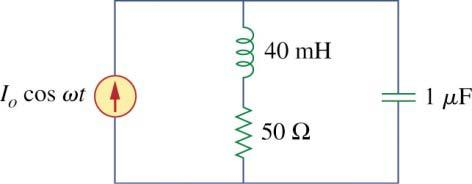
\includegraphics[width=2.48472in,height=1.14792in]{media/image2.jpeg}

\begin{quote}
Firstly, let us de ne what we already know about series RLC circuits.
\end{quote}

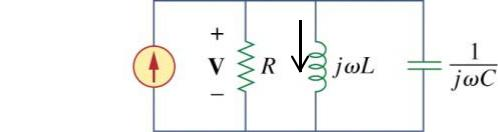
\includegraphics[width=3.43611in,height=1.98333in]{media/image3.jpeg}

\includegraphics[width=0.10139in,height=0.10139in]{media/image4.jpeg}

From the above equation for inductive reactance, if either the
\textbf{Frequency} or the \textbf{Inductance} is increased the overall
inductive reactance value of the inductor would also increase. As the
frequency approaches in nity the inductors reactance would also increase
towards in nity with the circuit element acting like an open circuit.

However, as the frequency approaches zero or DC, the inductors reactance
would decrease to zero, causing the opposite effect acting like a short
circuit. This means then that inductive reactance is
''\textbf{Proportional}'' to frequency and is small at low frequencies
and high at higher frequencies and this demonstrated in the following
curve:

\textbf{Inductive Reactance against Frequency}

\begin{quote}
The graph of inductive reactance against frequency is a straight line
linear curve. The inductive reactance value of an inductor increases
linearly as the frequency across it increases. Therefore, inductive
reactance is positive and is directly proportional to frequency (
$X_L \infty f$)
\end{quote}

\includegraphics[width=2.04167in,height=1.62708in]{media/image5.jpeg}

\begin{quote}
The same is also true for the capacitive reactance formula above but in
reverse. If either the \textbf{Frequency} or the \textbf{Capacitance} is
increased the overall capacitive reactance would decrease. As the
frequency approaches in nity the capacitors reactance would reduce to
zero causing the circuit element to act like a perfect conductor of
0Ω's.

But as the frequency approaches zero or DC level, the capacitors
reactance would rapidly increase up to in nity causing it to act like a
very large resistance acting like an open circuit condition. This means
then that capacitive reactance is ``\textbf{Inversely proportional}'' to
frequency for any given value of capacitance and this shown below:
\end{quote}

\textbf{Capacitive Reactance against Frequency}

\begin{quote}
The graph of capacitive reactance against frequency is a hyperbolic
curve. The Reactance value of a capacitor has a very high value at low
frequencies but quickly decreases as the frequency across it increases.
Therefore, capacitive reactance is negative and is inversely
proportional to frequency ( X\textsubscript{C} ∝ \textbf{ƒ}
\textsuperscript{-1} )
\end{quote}

\includegraphics[width=2.04167in,height=1.62014in]{media/image6.jpeg}

\begin{quote}
We can see that the values of these resistances depends upon the
frequency of the supply. At a higher frequency X\textsubscript{L} is
high and at a low frequency X\textsubscript{C} is high. Then there must
be a frequency point were the value of X\textsubscript{L} is the same as
the value of X\textsubscript{C} and there is. If we now place the curve
for inductive reactance on top of the curve for capacitive reactance so
that both curves are on the same axes, the point of intersection will
give us the series resonance frequency point, (
\textbf{ƒ}\textsubscript{r} or ω\textsubscript{r} ) as shown below.
\end{quote}

\textbf{Series Resonance Frequency}

\includegraphics[width=2.93472in,height=2.18681in]{media/image7.jpeg}

where: \textbf{f}\textsubscript{r} is in Hertz, L is in Henries and C is
in Farads.

Electrical resonance occurs in an AC circuit when the two reactances
which are opposite and equal cancel each other out as X\textsubscript{L}
= X\textsubscript{C} and the point on the graph at which this happens is
were the two reactance curves cross each other. In a series resonant
circuit, the resonant frequency, \textbf{ƒ}\textsubscript{r} point can
be calculated as follows.

\begin{quote}
We use cookies to enhance your experience. By continuing to visit this
site you agree to our use of cookies.
\href{http://wikipedia.org/wiki/HTTP_cookie}{More info}
\end{quote}

\includegraphics[width=0.10139in,height=0.10139in]{media/image8.jpeg}

\includegraphics[width=3.31250in,height=2.47014in]{media/image9.jpeg}

We can see then that at resonance, the two reactances cancel each other
out thereby making a series LC combination act as a short circuit with
the only opposition to current ow in a series resonance circuit being
the resistance, R. In complex form, the resonant frequency is the
frequency at which the total impedance of a series RLC circuit becomes
purely \emph{\textbf{``real''}}, that is no imaginary impedance's exist.
This is because at resonance they are cancelled out. So the total
impedance of the series circuit becomes just the value of the resistance
and therefore: Z = R.

Then at resonance the impedance of the series circuit is at its minimum
value and equal only to the resistance, R of the circuit. The circuit
impedance at resonance is called the ``dynamic impedance'' of the
circuit and depending upon the frequency, X\textsubscript{C} (typically
at high frequencies) or X\textsubscript{L} (typically at low
frequencies) will dominate either side of resonance as shown below.

\textbf{Impedance in a Series Resonance Circuit}

\includegraphics[width=2.57917in,height=2.19375in]{media/image10.jpeg}

Note that when the capacitive reactance dominates the circuit the
impedance curve has a hyperbolic shape to itself, but when the inductive
reactance dominates the circuit the curve is non-symmetrical due to the
linear response of X\textsubscript{L}. You may also note that if the
circuits impedance is at its minimum at resonance then consequently, the
circuits \textbf{admittance} must be at its maximum and one of the
characteristics of a series resonance circuit is that admittance is very
high. But this can be a bad thing because a very low value of resistance
at resonance means that the resulting current owing through the circuit
may be dangerously high.

We recall from the previous tutorial about series RLC circuits that the
voltage across a series combination is the phasor sum of
V\textsubscript{R}, V\textsubscript{L} and V\textsubscript{C}. Then if
at resonance the two reactances are equal and cancelling, the two
voltages representing V\textsubscript{L} and V\textsubscript{C} must
also be opposite and equal in value thereby cancelling each other out
because with pure components the phasor voltages are drawn at
+90\textsuperscript{o} and -90\textsuperscript{o} respectively.

Then in a \textbf{series resonance} circuit as V\textsubscript{L} =
-V\textsubscript{C} the resulting reactive voltages are zero and all the
supply voltage is dropped across the resistor. Therefore,

V\textsubscript{R} = V\textsubscript{supply} and it is for this reason
that series resonance circuits are known as voltage resonance circuits,
(as opposed to parallel resonance circuits which are current resonance
circuits).

\textbf{Series RLC Circuit at Resonance}

\begin{quote}
We use cookies to enhance your experience. By continuing to visit this
site you agree to our use of cookies.
\href{http://wikipedia.org/wiki/HTTP_cookie}{More info}
\end{quote}

\includegraphics[width=0.10139in,height=0.10139in]{media/image11.jpeg}

\includegraphics[width=4.03194in,height=1.65625in]{media/image12.jpeg}

Since the current owing through a series resonance circuit is the
product of voltage divided by impedance, at resonance the impedance, Z
is at its minimum value, ( =R ). Therefore, the circuit current at this
frequency will be at its maximum value of V/R as shown below.

\textbf{Series Circuit Current at Resonance}

\includegraphics[width=2.38264in,height=2.09236in]{media/image13.jpeg}

The frequency response curve of a series resonance circuit shows that
the magnitude of the current is a function of frequency and plotting
this onto a graph shows us that the response starts at near to zero,
reaches maximum value at the resonance frequency when
I\textsubscript{MAX} = I\textsubscript{R} and then drops again to nearly
zero as \textbf{ƒ} becomes in nite. The result of this is that the
magnitudes of the voltages across the inductor, L and the capacitor, C
can become many times larger than the supply voltage, even at resonance
but as they are equal and at opposition they cancel each other out.

As a series resonance circuit only functions on resonant frequency, this
type of circuit is also known as an \textbf{Acceptor Circuit} because at
resonance, the impedance of the circuit is at its minimum so easily
accepts the current whose frequency is equal to its resonant frequency.

You may also notice that as the maximum current through the circuit at
resonance is limited only by the value of the resistance (a pure and
real value), the source voltage and circuit current must therefore be in
phase with each other at this frequency. Then the phase angle between
the voltage and current of a series resonance circuit is also a function
of frequency for a xed supply voltage and which is zero at the resonant
frequency point when: V, I and V\textsubscript{R} are all in phase with
each other as shown below. Consequently, if the phase angle is zero then
the power factor must therefore be unity.

\textbf{Phase Angle of a Series Resonance Circuit}

\begin{quote}
We use cookies to enhance your experience. By continuing to visit this
site you agree to our use of cookies.
\href{http://wikipedia.org/wiki/HTTP_cookie}{More info}
\end{quote}

\includegraphics[width=0.10139in,height=0.10139in]{media/image14.jpeg}

\includegraphics[width=4.10486in,height=3.10972in]{media/image15.jpeg}

Notice also, that the phase angle is positive for frequencies above
\textbf{ƒ}\textsubscript{r} and negative for frequencies below
\textbf{ƒ}\textsubscript{r} and this can be proven by,

\includegraphics[width=2.47014in,height=0.40694in]{media/image16.jpeg}

\textbf{Bandwidth of a Series Resonance Circuit}

If the series RLC circuit is driven by a variable frequency at a
constant voltage, then the magnitude of the current, I is proportional
to the impedance, Z, therefore at resonance the power absorbed by the
circuit must be at its maximum value as P = I\textsuperscript{2}Z.

If we now reduce or increase the frequency until the average power
absorbed by the resistor in the series resonance circuit is half that of
its maximum value at resonance, we produce two frequency points called
the \textbf{half-power points} which are -3dB down from maximum, taking
0dB as the maximum current reference.

These -3dB points give us a current value that is 70.7\% of its maximum
resonant value which is de ned as: 0.5( I\textsuperscript{2} R ) =
(0.707 x I)\textsuperscript{2} R. Then the point corresponding to the
lower frequency at half the power is called the ``lower cut-off
frequency'', labelled \textbf{ƒ}\textsubscript{L} with the point
corresponding to the upper frequency at half power being called the
``upper cut-off frequency'', labelled \textbf{ƒ}\textsubscript{H}. The
distance between these two points, i.e. ( \textbf{ƒ}\textsubscript{H} --
\textbf{ƒ}\textsubscript{L} ) is called the \textbf{Bandwidth}, (BW) and
is the range of frequencies over which at least half of the maximum
power and current is provided as shown.

\textbf{Bandwidth of a Series Resonance Circuit}

\includegraphics[width=2.73889in,height=2.28819in]{media/image17.jpeg}

The frequency response of the circuits current magnitude above, relates
to the ``sharpness'' of the resonance in a series resonance circuit. The
sharpness of the peak is measured quantitatively and is called the
\textbf{Quality factor, Q} of the circuit. The quality factor relates
the maximum or peak energy stored in the circuit (the reactance) to the
energy dissipated (the resistance) during each cycle of oscillation
meaning that it is a ratio of resonant frequency to bandwidth and the
higher the circuit Q, the smaller the bandwidth, Q =
\textbf{ƒ}\textsubscript{r} /BW.

\begin{quote}
We use cookies to enhance your experience. By continuing to visit this
site you agree to our use of cookies.
\href{http://wikipedia.org/wiki/HTTP_cookie}{More info}
\end{quote}

\includegraphics[width=0.10139in,height=0.10139in]{media/image18.jpeg}

As the bandwidth is taken between the two -3dB points, the
\textbf{selectivity} of the circuit is a measure of its ability to
reject any frequencies either side of these points. A more selective
circuit will have a narrower bandwidth whereas a less selective circuit
will have a wider bandwidth. The selectivity of a series resonance
circuit can be controlled by adjusting the value of the resistance only,
keeping all the other components the same, since Q = (X\textsubscript{L}
or X\textsubscript{C})/R.

\textbf{Bandwidth of a Series RLC Resonance Circuit}

\includegraphics[width=2.37569in,height=1.99028in]{media/image19.jpeg}

Then the relationship between resonance, bandwidth, selectivity and
quality factor for a series resonance circuit being de ned as:

1). Resonant Frequency, (\textbf{ƒ}\textsubscript{r})

\includegraphics[width=2.44861in,height=1.08264in]{media/image20.jpeg}

2). Current, (I)

\includegraphics[width=3.71944in,height=1.22083in]{media/image21.jpeg}

3). Lower cut-off frequency, (\textbf{ƒ}\textsubscript{L})

\includegraphics[width=3.02222in,height=1.86736in]{media/image22.jpeg}

4). Upper cut-off frequency, (\textbf{ƒ}\textsubscript{H})

\begin{quote}
We use cookies to enhance your experience. By continuing to visit this
site you agree to our use of cookies.
\href{http://wikipedia.org/wiki/HTTP_cookie}{More info}
\end{quote}

\includegraphics[width=0.10139in,height=0.10139in]{media/image23.jpeg}

\includegraphics[width=3.02222in,height=1.87431in]{media/image24.jpeg}

5). Bandwidth, (BW)

\includegraphics[width=3.54514in,height=0.43611in]{media/image25.jpeg}

6). Quality Factor, (Q)

\includegraphics[width=2.83333in,height=0.46528in]{media/image26.jpeg}

\textbf{Series Resonance Example No1}

A series resonance network consisting of a resistor of 30Ω, a capacitor
of 2uF and an inductor of 20mH is connected across a sinusoidal supply
voltage which has a constant output of 9 volts at all frequencies.
Calculate, the resonant frequency, the current at resonance, the voltage
across the inductor and capacitor at resonance, the quality factor and
the bandwidth of the circuit. Also sketch the corresponding current
waveform for all frequencies.

\includegraphics[width=2.48472in,height=1.37292in]{media/image27.jpeg}

Resonant Frequency, \textbf{ƒ}\textsubscript{r}

\includegraphics[width=3.17500in,height=0.50139in]{media/image28.jpeg}

Circuit Current at Resonance, I\textsubscript{m}

\includegraphics[width=2.44861in,height=0.37778in]{media/image29.jpeg}

Inductive Reactance at Resonance, X\textsubscript{L}

\includegraphics[width=2.81875in,height=0.23958in]{media/image30.jpeg}

Voltages across the inductor and the capacitor, V\textsubscript{L},
V\textsubscript{C}

\begin{quote}
We use cookies to enhance your experience. By continuing to visit this
site you agree to our use of cookies.
\href{http://wikipedia.org/wiki/HTTP_cookie}{More info}
\end{quote}

\includegraphics[width=0.10139in,height=0.10139in]{media/image31.jpeg}

\includegraphics[width=2.13611in,height=0.73403in]{media/image32.jpeg}

Note: the supply voltage may be only 9 volts, but at resonance, the
reactive voltages across the capacitor, V\textsubscript{C} and the
inductor, V\textsubscript{L} are 30 volts peak! Quality factor, Q

\includegraphics[width=1.72153in,height=0.41389in]{media/image33.jpeg}

Bandwidth, BW

\includegraphics[width=2.21597in,height=0.40694in]{media/image34.jpeg}

The upper and lower -3dB frequency points, \textbf{ƒ}\textsubscript{H}
and \textbf{ƒ}\textsubscript{L}

\includegraphics[width=3.31250in,height=0.98819in]{media/image35.jpeg}

Current Waveform

\includegraphics[width=2.95694in,height=2.47014in]{media/image36.jpeg}

\textbf{Series Resonance Example No2}

A series circuit consists of a resistance of 4Ω, an inductance of 500mH
and a variable capacitance connected across a 100V, 50Hz supply.
Calculate the capacitance require to produce a series resonance
condition, and the voltages generated across both the inductor and the
capacitor at the point of resonance.

Resonant Frequency, \textbf{ƒ}\textsubscript{r}

\includegraphics[width=3.00069in,height=1.35139in]{media/image37.jpeg}

Voltages across the inductor and the capacitor, V , V

We use cookies to enhance your experienceLC. By continuing to visit this
site you agree to our use of cookies.
\href{http://wikipedia.org/wiki/HTTP_cookie}{More info}

\includegraphics[width=0.10139in,height=0.10139in]{media/image38.jpeg}

\includegraphics[width=2.55694in,height=1.78750in]{media/image39.jpeg}

\begin{quote}
\textbf{Series Resonance Summary}

You may have noticed that during the analysis of series resonance
circuits in this tutorial, we looked at bandwidth, upper and lower
frequencies, -3dB points and quality or Q-factor. All these are terms
used in designing and building of Band Pass Filters (BPF) and indeed,
resonance circuits are used in 3-element mains lter designs to pass all
frequencies within the ``passband'' range while rejecting all others.

However, the main aim of this tutorial is to analyse and understand the
concept of how \textbf{Series Resonance} occurs in passive RLC series
circuits. Their use in RLC lter networks and designs is outside the
scope of this particular tutorial, and so will not be looked at here,
sorry.

For resonance to occur in any circuit it must have at least one inductor
and one capacitor.
\end{quote}

\includegraphics{media/image40.jpeg}

\begin{quote}
Resonance is the result of oscillations in a circuit as stored energy is
passed from the inductor to the capacitor.
\end{quote}

\includegraphics{media/image41.jpeg}

\begin{quote}
Resonance occurs when X\textsubscript{L} = X\textsubscript{C} and the
imaginary part of the transfer function is zero.
\end{quote}

\includegraphics{media/image42.jpeg}

\begin{quote}
At resonance the impedance of the circuit is equal to the resistance
value as Z = R.
\end{quote}

\includegraphics{media/image43.jpeg}

\begin{quote}
At low frequencies the series circuit is capacitive as:
X\textsubscript{C} \textgreater{} X\textsubscript{L}, this gives the
circuit a leading power factor.
\end{quote}

\includegraphics{media/image44.jpeg}

\begin{quote}
At high frequencies the series circuit is inductive as:
X\textsubscript{L} \textgreater{} X\textsubscript{C}, this gives the
circuit a lagging power factor.
\end{quote}

\includegraphics{media/image45.jpeg}

\begin{quote}
The high value of current at resonance produces very high values of
voltage across the inductor and capacitor.
\end{quote}

\includegraphics{media/image46.jpeg}

\begin{quote}
Series resonance circuits are useful for constructing highly frequency
selective lters. However, its high current and very high component
voltage values can cause damage to the circuit.
\end{quote}

\includegraphics{media/image47.jpeg}

\begin{quote}
The most prominent feature of the frequency response of a resonant
circuit is a sharp resonant peak in its amplitude characteristics.
\end{quote}

\includegraphics{media/image48.jpeg}

\begin{quote}
Because impedance is minimum and current is maximum, series resonance
circuits are also called \textbf{Acceptor Circuits}.
\end{quote}

\includegraphics{media/image49.jpeg}

\begin{quote}
In the next tutorial about Parallel Resonance we will look at how
frequency affects the characteristics of a parallel connected RLC
circuit and how this time the Q-factor of a parallel resonant circuit
determines its current magni cation.
\end{quote}

\textbf{103 Comments}

\includegraphics[width=8.28194in]{media/image50.jpeg}

\begin{quote}
Join the conversation!
\end{quote}

\includegraphics[width=7.91806in,height=0.36250in]{media/image51.jpeg}

\begin{quote}
Your Name
\end{quote}

\includegraphics[width=7.91806in,height=0.36250in]{media/image52.jpeg}

\begin{quote}
Email Address

We use cookies to enhance your experience. By continuing to visit this
site you agree to our use of cookies.
\href{http://wikipedia.org/wiki/HTTP_cookie}{More info}
\end{quote}

\includegraphics[width=0.10139in,height=0.10139in]{media/image53.jpeg}

\begin{quote}
\includegraphics[width=7.91806in,height=1.75764in]{media/image54.jpeg}
\end{quote}

SUBMIT

\begin{itemize}
\item
  \begin{quote}
  Pierre
  \end{quote}
\end{itemize}

\begin{quote}
I want some help please.

Posted on \protect\hyperlink{page10}{January 16th 2018 \textbar{} 5:16
pm}

\href{https://www.electronics-tutorials.ws/accircuits/series-resonance.html?replytocom=47334\#respond}{Reply}
\end{quote}

\includegraphics[width=8.28194in]{media/image55.jpeg}

\begin{itemize}
\item
  \begin{quote}
  RAHIM
  \end{quote}
\end{itemize}

\begin{quote}
hi\ldots{}

i wonder does the current at resonance equal tu peak current across the
resistor or it is equal to root mean square current across resistor

Posted on \protect\hyperlink{page10}{December 27th 2017 \textbar{} 2:27
am}

\href{https://www.electronics-tutorials.ws/accircuits/series-resonance.html?replytocom=45585\#respond}{Reply}
\end{quote}

\includegraphics[width=8.28194in]{media/image56.jpeg}

\begin{itemize}
\item
  \begin{quote}
  Colline
  \end{quote}
\end{itemize}

\begin{quote}
Could you help me to work out why the dynamic impedance increases as the
LC ratio changes.at 7 megahertz if you have 14pf and around
30microheneries the dynamic Z is around 20 ohms but if you make C
smaller and L 60 microheneries the Dynamic Z is over 100 ohms. Why is
this please.

Posted on \protect\hyperlink{page10}{December 18th 2017 \textbar{} 10:13
pm}

\href{https://www.electronics-tutorials.ws/accircuits/series-resonance.html?replytocom=44972\#respond}{Reply}
\end{quote}

\includegraphics[width=8.28194in]{media/image57.jpeg}

\begin{itemize}
\item
  Deepak Srivastava
\end{itemize}

\begin{quote}
Very nice\ldots{}

Great explanation

Posted on \protect\hyperlink{page10}{December 15th 2017 \textbar{} 1:42
pm}
\end{quote}

\includegraphics[width=8.28194in]{media/image58.jpeg}

\begin{itemize}
\item
  \begin{quote}
  Sandy Cheeks
  \end{quote}
\end{itemize}

\begin{quote}
I like Bread ngers

Posted on \protect\hyperlink{page10}{December 11th 2017 \textbar{} 11:48
am}

We use cookies to enhance your experience. By continuing to visit this
site you agree to our use of cookies.
\href{http://wikipedia.org/wiki/HTTP_cookie}{More info}
\end{quote}

\href{https://www.electronics-tutorials.ws/accircuits/series-resonance.html?replytocom=44696\#respond}{Reply}

\href{https://www.electronics-tutorials.ws/accircuits/series-resonance.html?replytocom=44325\#respond}{Reply}

\includegraphics[width=0.10139in,height=0.10139in]{media/image59.jpeg}

\begin{itemize}
\item
  \begin{quote}
  \includegraphics[width=8.28194in]{media/image60.jpeg}
  \end{quote}
\end{itemize}

\begin{quote}
Thanks..
\end{quote}

Posted on \protect\hyperlink{page11}{December 07th 2017 \textbar{} 3:06
am}

\begin{quote}
\href{https://www.electronics-tutorials.ws/accircuits/series-resonance.html?replytocom=43874\#respond}{Reply}
\end{quote}

\includegraphics[width=8.28194in]{media/image61.jpeg}

\begin{itemize}
\item
  Muhammad Ali Haider
\end{itemize}

\begin{quote}
Very nice article, learned a lot from it but still have confusion in
Half power frequencies.

Posted on \protect\hyperlink{page11}{December 04th 2017 \textbar{} 2:33
pm}

\href{https://www.electronics-tutorials.ws/accircuits/series-resonance.html?replytocom=43583\#respond}{Reply}
\end{quote}

\includegraphics[width=8.28194in]{media/image62.jpeg}

\begin{itemize}
\item
  \begin{quote}
  Sebastian
  \end{quote}
\end{itemize}

thank you very much you just saved me from failing

\begin{quote}
Posted on \protect\hyperlink{page11}{November 29th 2017 \textbar{} 11:36
pm}

\href{https://www.electronics-tutorials.ws/accircuits/series-resonance.html?replytocom=43063\#respond}{Reply}
\end{quote}

\includegraphics[width=8.28194in]{media/image63.jpeg}

\begin{itemize}
\item
  \begin{quote}
  Bharathi
  \end{quote}
\end{itemize}

\begin{quote}
nice explanation
\end{quote}

Posted on \protect\hyperlink{page11}{November 23rd 2017 \textbar{} 12:23
pm}

\begin{quote}
\href{https://www.electronics-tutorials.ws/accircuits/series-resonance.html?replytocom=42169\#respond}{Reply}
\end{quote}

\includegraphics[width=8.28194in]{media/image64.jpeg}

\begin{itemize}
\item
  \begin{quote}
  BharathI
  \end{quote}
\end{itemize}

\begin{quote}
Nice
\end{quote}

Posted on \protect\hyperlink{page11}{November 23rd 2017 \textbar{} 12:21
pm}

\begin{quote}
\href{https://www.electronics-tutorials.ws/accircuits/series-resonance.html?replytocom=42168\#respond}{Reply}
\end{quote}

\includegraphics[width=8.28194in]{media/image65.jpeg}

\begin{quote}
\href{https://www.electronics-tutorials.ws/accircuits/series-resonance.html/comment-page-2\#comments}{View
More}

We use cookies to enhance your experience. By continuing to visit this
site you agree to our use of cookies.
\href{http://wikipedia.org/wiki/HTTP_cookie}{More info}
\end{quote}

\includegraphics[width=0.10139in,height=0.10139in]{media/image67.jpeg}

\end{document}
